Visualisation is not a new phenomenon. It has been used in maps, scientific drawings, and data plots for over a thousand years \iacite{Friendly.2001}. Examples of this are the map of China and the famous map of Napoleon's invasion of Russia which are explained later in detail. Most of the concepts learned in devising these images carry over in a straightforward manner to computer visualisation \iacite{Tufte:1990}.

The first part of this section provides an overview of significant milestones in the history of visualisation. It is followed by a definition of visualisation in literature and a varieties of visualisation for this thesis, yielding to the basis to be able to define different types of visualisation like \ac{InfoVis}, \ac{SciVis} and \ac{GeoVis} (which are all explained in detail in section \ref{s:definitions-types} on page \pageref{s:definitions-types}). The definitions are followed by an essential discussion about the basic principles of data visualisations and differnet types of visualisations.

The second part of this section uses the knowledge of the first part to describe exploratory data analysis in conjunction with visualisations. This is also done with some practical applications and examples which are also used to segue into the next chapter which deals with \ac{GeoVis}. It is used to show different types and use cases of \ac{GeoVis}.

\subsubsection{History}
\label{s:history}
This entire chapter is based on the work of \citeauthor{Friendly.2001}, who made an interactive timeline of milestones of the history of visualizatoins. Even though \citeauthor{Friendly.2001} provide a huge amount of historical visualizations and informations, it is not possible to discuss and mention everything because it would go beyond the scope and therefore only the important visualizations for this thesis are used \iacite{Friendly.2001}.

\begin{quote}
    The earliest seeds of visualization arose in geometric diagrams, in tables of the positions of stars and other celestial bodies, and in the making of maps to aid in navigation and exploration \iacite{Friendly.2001}.
\end{quote}

In 1508 a map of the Roman empire came in the way of Konrad Peutinger. This map was named after him at a later date: Tabula Peutingeriana or Peutinger map. Before Peutinger got the map it was copied from an old roman world map from the 4\textsuperscript{th} century A.D, which in turn was copied from the world map of Agrippina (from the 1\textsuperscript{st} century B.C.). Figure \ref{fig:peutinger} on page \pageref{fig:peutinger} shows the peutinger map which had a length of 680cm and was drawn on a long book-roll.

\begin{figure}[!htb]
\centering
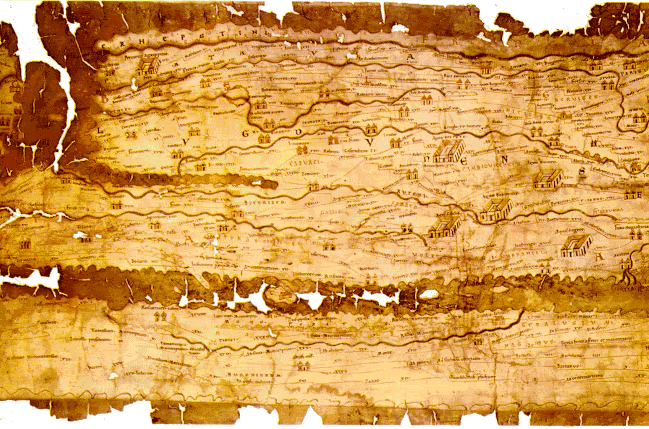
\includegraphics[width=0.8\textwidth,keepaspectratio]{images/history/peutinger.png}
\caption[
    Peutinger map, Urldate: 07.2016 \newline
\small\texttt{\url{https://web.archive.org/web/20080129123649/http://www.kargi.de/Geschichte/Peutinger/Peutinger.bmp}}
]{Peutinger map}
\label{fig:peutinger}
\end{figure}

Figure \ref{fig:peutinger-rome} on page \pageref{fig:peutinger-rome} shows Rome as the central point with 12 different ways leaving it. The map was not meant to be accurate and true to scale. Its main goal was to give travelers outline where they need to go to reach their destination. All distances in the map are graphically distorted but the correct distances are mentioned next to the roads as numbers. Thus the map
s only accuracy consists of the structure (left and right).

\begin{figure}[!htb]
\centering
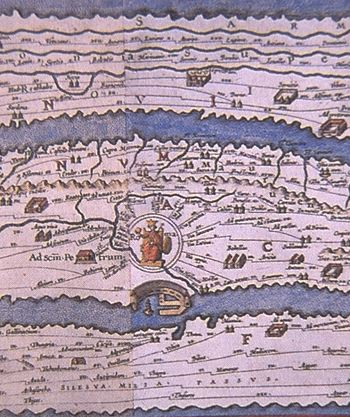
\includegraphics[width=0.5\textwidth,keepaspectratio]{images/history/peutinger_rom.jpg}
\caption[
    Peutinger map with Rome as central point, Urldate: 07.2016 \newline
\small\texttt{\url{https://web.archive.org/web/20060106224928/http://www.kargi.de/Geschichte/Peutinger/peutinger_rom.jpg}}
]{Peutinger map with Rome as central point}
\label{fig:peutinger-rome}
\end{figure}

A greek astronomer called Ptolemy was one of the most influential greek astronomers and geographers of his time. He was one of the first to propound the geocentric theory of the solar system. His maps used a projection of a spherical earth and latitude together with longitude to characterize position. Alongside the first use of longitude in maps he also was the first one specifying terrestrial ocations by celestial observations. Figure \ref{fig:ptolemy} on page \pageref{fig:ptolemy} shows a reconstructed map from Ptolemy's geohraphy in the 15\textsuperscript{th} century, indicating "Sinae" at the far right, beyond the oversized island of "Taprobane" and the "Aurea Chersonesus".

\begin{figure}[!htb]
\centering
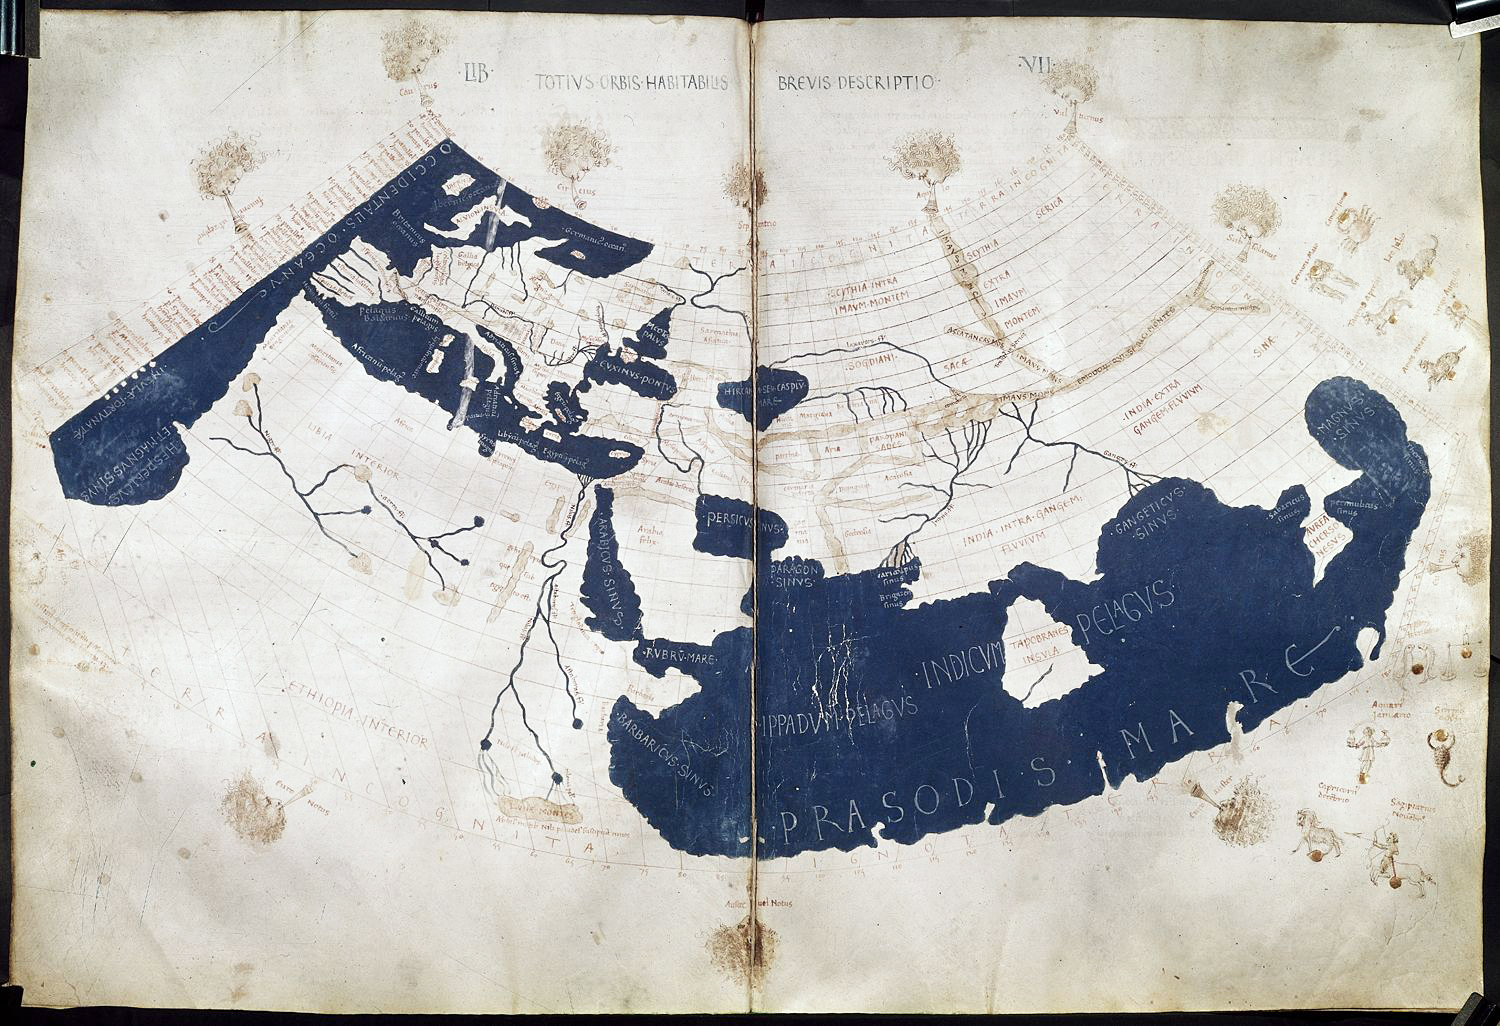
\includegraphics[width=0.6\textwidth,keepaspectratio]{images/history/ptolemy-map.jpg}
\caption[
    Reconstructed Ptolemy's map, Urldate: 07.2016 \newline
\small\texttt{\url{https://upload.wikimedia.org/wikipedia/commons/2/23/PtolemyWorldMap.jpg}}
]{Reconstructed Ptolemy's map}
\label{fig:ptolemy}
\end{figure}

The earliest known attempt to show changing values graphically was around the 10\textsuperscript{th} century. Figure \ref{fig:planetary-movement} on page \pageref{fig:planetary-movement} tries to show planetary
movement like the positions of the sun, moon and planets throughout the year.

\begin{figure}[!htb]
\centering
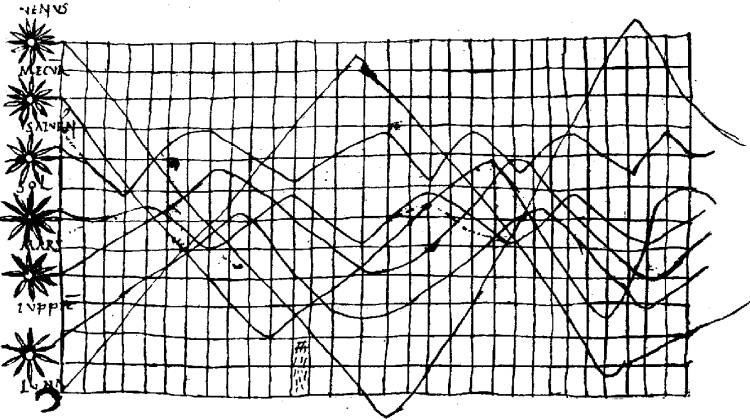
\includegraphics[width=0.4\textwidth,keepaspectratio]{images/history/planetary-movement.jpg}
\caption[
    Planetary movements, Urldate: 07.2016 \newline
\small\texttt{\url{http://www.fi.uu.nl/wiskrant/artikelen/hist_grafieken/begin/images/planeten.gif}}
]{Planetary movements}
\label{fig:planetary-movement}
\end{figure}

1350 was the year in which the first bar chart of its sort appeared and was named proto-bar graph. Oresme, a french bishop and philosopher, proposed the use of a bar graph for plotting a variable magnitude whose value depends on another. Figure \ref{fig:oresme-proto} on \pageref{fig:oresme-proto} shows such a graph in detail and figure \ref{fig:oresme-page} on \pageref{fig:oresme-page} shows a page written in Latin containing different types of concepts which all implicitly have the idea of a coordinate system. The graphical use of bars also reveal the implication of the use of mathematical aggregation.

\begin{figure}[!htb]
\centering
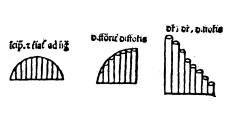
\includegraphics[height=4cm,keepaspectratio]{images/history/oresme-proto.jpg}
\caption[
    Oresme proto bar graph, Urldate: 07.2016 \newline
\small\texttt{\url{http://datavis.ca/milestones//admin/uploads/images/icons/oresmekl.gif}}
]{Oresme proto bar graph}
\label{fig:oresme-proto}
\end{figure}

\begin{figure}[!htb]
\centering
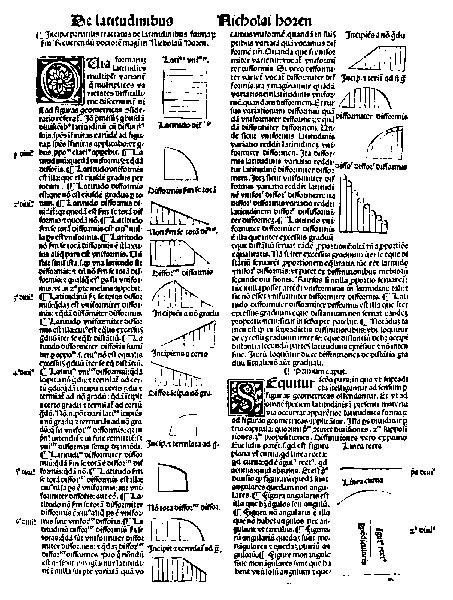
\includegraphics[height=10cm,keepaspectratio]{images/history/oresme-page.jpg}
\caption[
    Oresmes concept page written in Latin, Urldate: 07.2016 \newline
\small\texttt{\url{http://datavis.ca/milestones//admin/uploads/images/oresme6.gif}}
]{Oresmes concept page written in Latin}
\label{fig:oresme-page}
\end{figure}

25 years later, 1375, Abraham and Jehuda Cresques made the first catalan atlas. It consists of six images also called portulan charts which show the position of coasts and ports very accurately. All portulan charts together cover the regions from the Atlantic Ocean to China. The informations to make the atlas was gathered from sailors who used Mallorca, the hometown of Abraham and Jehuda Cresques, as a junction. Figure \ref{fig:catalan-atlas} on page \pageref{fig:catalan-atlas} shows one portulan chart displaying Europe, North Africa and the Near East. The atlas was the first of its kind having undistorted distances between geographical regions.

\begin{figure}[!htb]
\centering
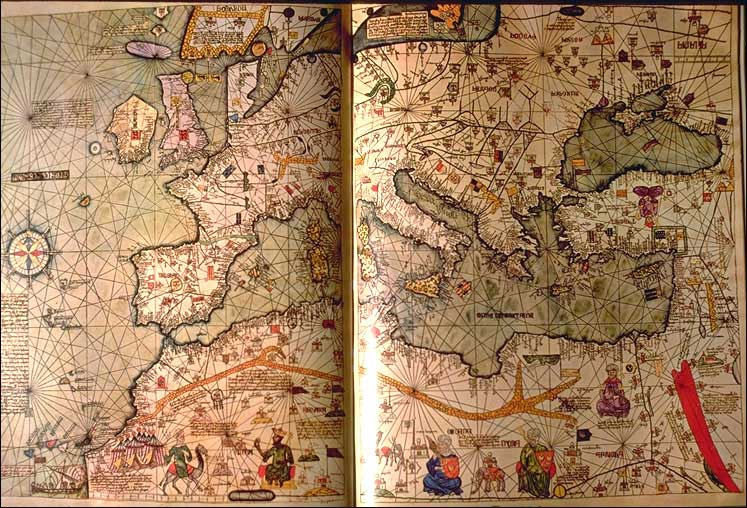
\includegraphics[width=0.8\textwidth,keepaspectratio]{images/history/catalan-atlas.jpg}
\caption[
    One out of six portulan charts of the catalan atlas, Urldate: 07.2016 \newline
\small\texttt{\url{http://datavis.ca/milestones//admin/uploads/images/CatalanE.jpg}}
]{One out of six portulan charts of the catalan atlas}
\label{fig:catalan-atlas}
\end{figure}

1569 Gerard Mercator invented a new map projection which bears his name. The main task for this projection was to map a world on to a cylinder in such a way that all lines of latitude have the same length as the equator. This should help seamen to lay out a course easily because a nagivator needed a map where a line of constant bearing would cross all meridians at the same angle. On the one hand the projection provides very accurate directions and shapes of regions, but on the other hand the size of regions are distorted incresingly to the north and south pole. Figure \ref{fig:mercator} on page \pageref{fig:mercator} shows a map of the world with a mercator projection.

\begin{figure}[!htb]
\centering
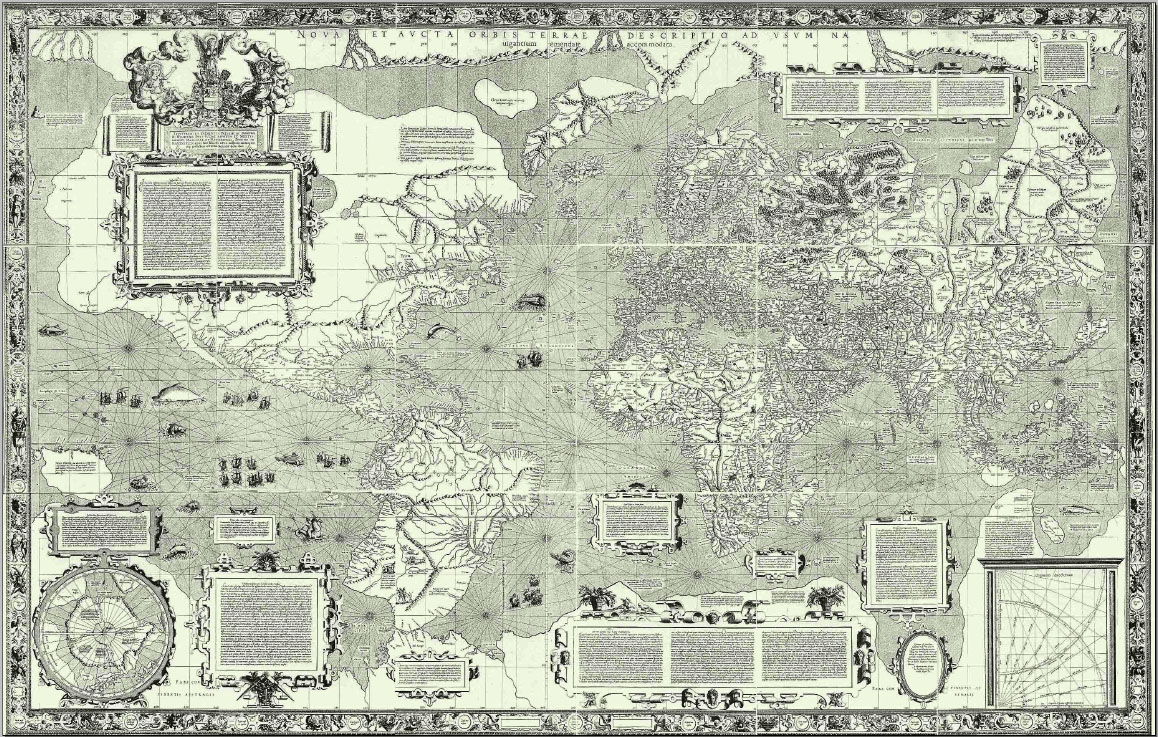
\includegraphics[width=0.8\textwidth,keepaspectratio]{images/history/mercator.png}
\caption[
    A map of the world with a mercator projection, Urldate: 07.2016 \newline
\small\texttt{\url{https://upload.wikimedia.org/wikipedia/commons/b/b2/Mercator_1569.png}}
]{A map of the world with a mercator projection}
\label{fig:mercator}
\end{figure}

One year later, 1570, the first modern atlas named Teatrum Orbis Terrarum ("Theatre of the World"), or Ortelius-Atlas appeared. It was a book consisting of a collection of uniform map sheets and sustaining text bounds. The collection of map sheets contained actually no maps from the hand of Orelius. At first it bundled maps from 53 other cartographers with the source. However Ortelius brought consistency to all those maps. He dropped the maps all in the same style and size and arranged them logically by continent, region and state. Nevertheless the naming and location coordinates were not normalized. Figure \ref{fig:ortelius} on \pageref{fig:ortelius} shows a world map in Teatrum Orbis Terrarum. Ortelius also regularly revised and expanded the atlas making it the first economically successful one.

\begin{figure}[!htb]
\centering
\includegraphics[width=0.8\textwidth,keepaspectratio]{images/history/ortelius.jpeg}
\caption[
    A map of the world in the Ortelius atlas, Urldate: 07.2016 \newline
\small\texttt{\url{https://upload.wikimedia.org/wikipedia/commons/6/6f/OrteliusWorldMap.jpeg}}
]{A map of the world in the Ortelius atlas}
\label{fig:ortelius}
\end{figure}

1626 the idea of "small multiples" got developed. It was used to show a series of images in a coherent display. The origin of the idea is based in displaying the changes in sunspots over time in a visual representation as figure \ref{fig:small-multiples} on page \pageref{fig:small-multiples} shows.

\begin{figure}[!htb]
\centering
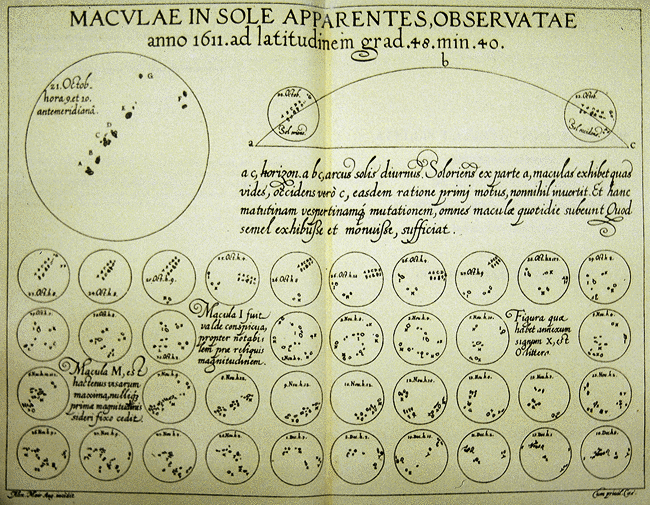
\includegraphics[height=5cm,keepaspectratio]{images/history/small-multiples.png}
\caption[
    Sunspot plate from Scheiner's "Tres Epistolae" using small multiples, Urldate: 07.2016 \newline
\small\texttt{\url{http://cnx.rice.edu/content/m11970/latest/tres_epistolae.gif}}
]{Sunspot plate from Scheiner's "Tres Epistolae" using small multiples}
\label{fig:small-multiples}
\end{figure}

20 years later the first visual representation of statistical data was made. Langren showed the variations in determination of longitude between Toledo and Rome (see figure \ref{fig:langren} on page \pageref{fig:langren}).

\begin{figure}[!htb]
\centering
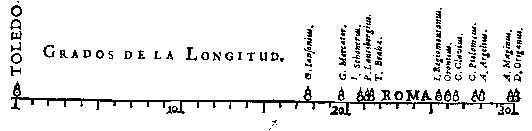
\includegraphics[width=0.8\textwidth,keepaspectratio]{images/history/langren.jpg}
\caption[
    First data graph showing variations in determination of longitude between Toledo and Rome, Urldate: 07.2016 \newline
\small\texttt{\url{http://datavis.ca/milestones//admin/uploads/images/tufte/langren.jpg}}
]{First data graph showing variations in determination of longitude between Toledo and Rome}
\label{fig:langren}
\end{figure}

In the 18\textsuperscript{th} century, cartographers began to try to show more than one channel on a map. Up to now the only channel which got displayed on a map was just geographical position. As a result, new graphic forms such as contours lines, or also called isolines, got invented and thematic mapping of physical quantities took root. Towards the end of this century, the first attempts at thematic mapping of geologic, economic, and medical data are visible.

The first half of the 19\textsuperscript{th} century witnessed a tremendous growth in statistical graphics and thematic mapping because of the fertilization provided by previous innovations of design and technique. All modern forms of data visualizations now known as bar and pie charts, histograms, line graphs and time-series plots, contour plots and so forth, werde invented. In the field of cartography, a shift from single geographical maps to comprehensive atlases, depicting data on a wide variety of topics (economic, social, medical, physcical, etc.) happened. As an example, figure \ref{fig:first-choropleth} on page \pageref{fig:first-choropleth} shows the first choropleth map. It shows the distribution and intensity of illiteracy in France.

\begin{figure}[!htb]
\centering
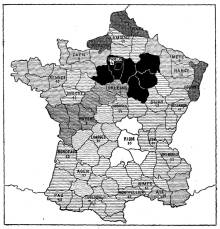
\includegraphics[height=5cm,keepaspectratio]{images/history/dupin.jpg}
\caption[
    First choropleth map showing the distribution and intensity of illiteracy in France, Urldate: 07.2016 \newline
\small\texttt{\url{http://datavis.ca/milestones//admin/uploads/images/dupin.gif}}
]{First choropleth map showing the distribution and intensity of illiteracy in France}
\label{fig:first-choropleth}
\end{figure}

This map was followed shortly by comparative choropleth thematic maps, showing crimes against persons and crimes against property in relation to level of instruction by departments in France (see figure \ref{fig:second-choropleth} on page \pageref{fig:second-choropleth}.).

\begin{figure}[!htb]
\centering
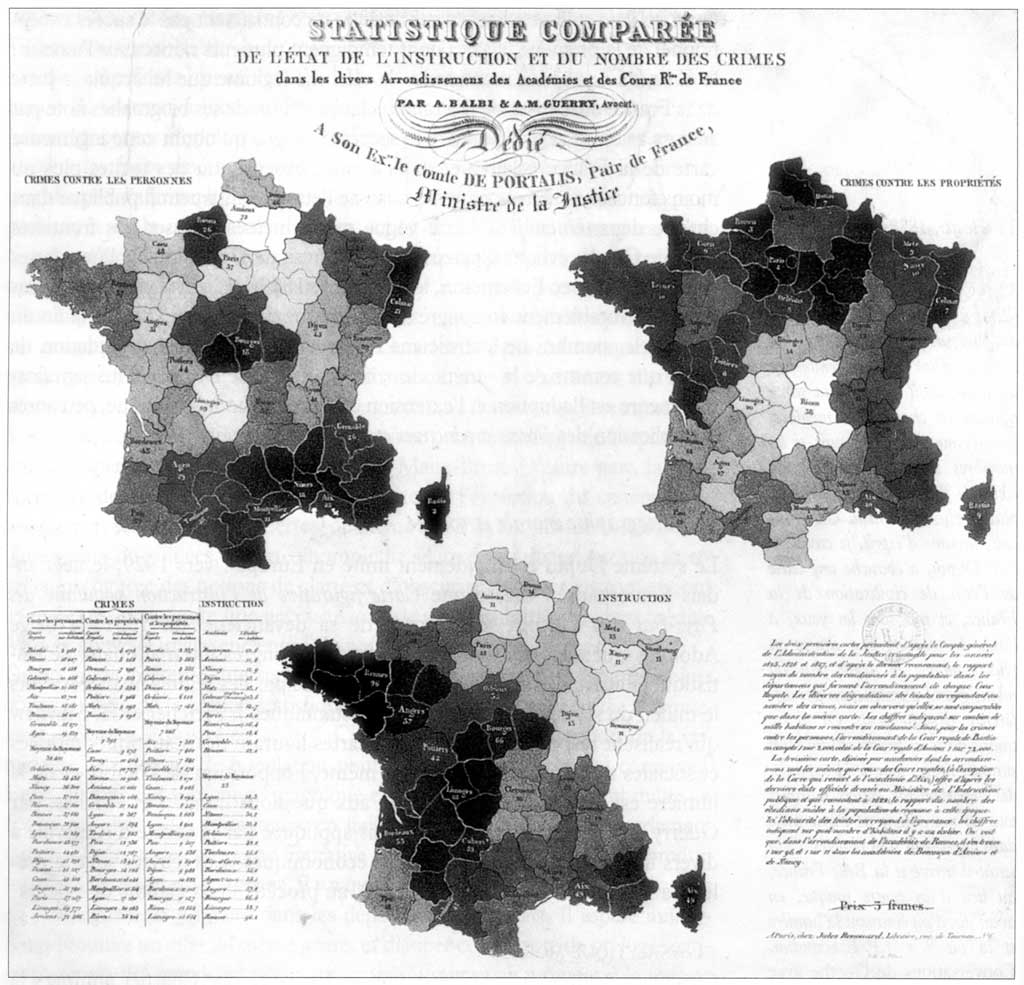
\includegraphics[height=5cm,keepaspectratio]{images/history/second-choropleth.jpg}
\caption[
    The first comparative choropleth thematic maps, showing crimes against persons and crimes against property in relation to level of instruction by departments in France, Urldate: 07.2016 \newline
\small\texttt{\url{http://datavis.ca/milestones//admin/uploads/images/guerry/guerry-balbi-600s.jpg}}
]{The first comparative choropleth thematic maps, showing crimes against persons and crimes against property in relation to level of instruction by departments in France}
\label{fig:second-choropleth}
\end{figure}

1830 the first dot map of population appeared in France. Each dot represents 10.000 people in the department (see figure \ref{fig:first-dotmap} on page \pageref{fig:first-dotmap}.).

\begin{figure}[!htb]
\centering
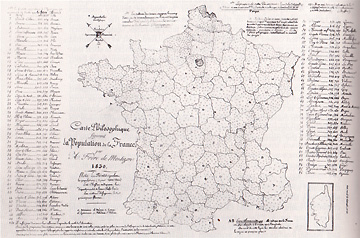
\includegraphics[width=0.8\textwidth,keepaspectratio]{images/history/montizon-dotmap.jpg}
\caption[
    The first dot map of population by department, 1 dot = 10.000 people, Urldate: 07.2016 \newline
\small\texttt{\url{http://datavis.ca/milestones//admin/uploads/images/montizon-dotmap.jpg}}
]{The first dot map of population by department, 1 dot = 10.000 people}
\label{fig:first-dotmap}
\end{figure}

The second half of the 19\textsuperscript{th} century is also known as "the golden age of data graphics". All the conditions for tremendous growth of visualizations were given once again: throughout Europe official state statistical offices were established.
Statistical theory (initiated by Gauss and Laplace) provided the means to make sense of large bodies of data.
This half of the century included the first mixture of a map with a diagram: figure \ref{fig:first-mixture} on page \pageref{fig:first-mixture} shows a map using pie charts to represent the cattle sent from all around France for consumption in Paris.

\begin{figure}[!htb]
\centering
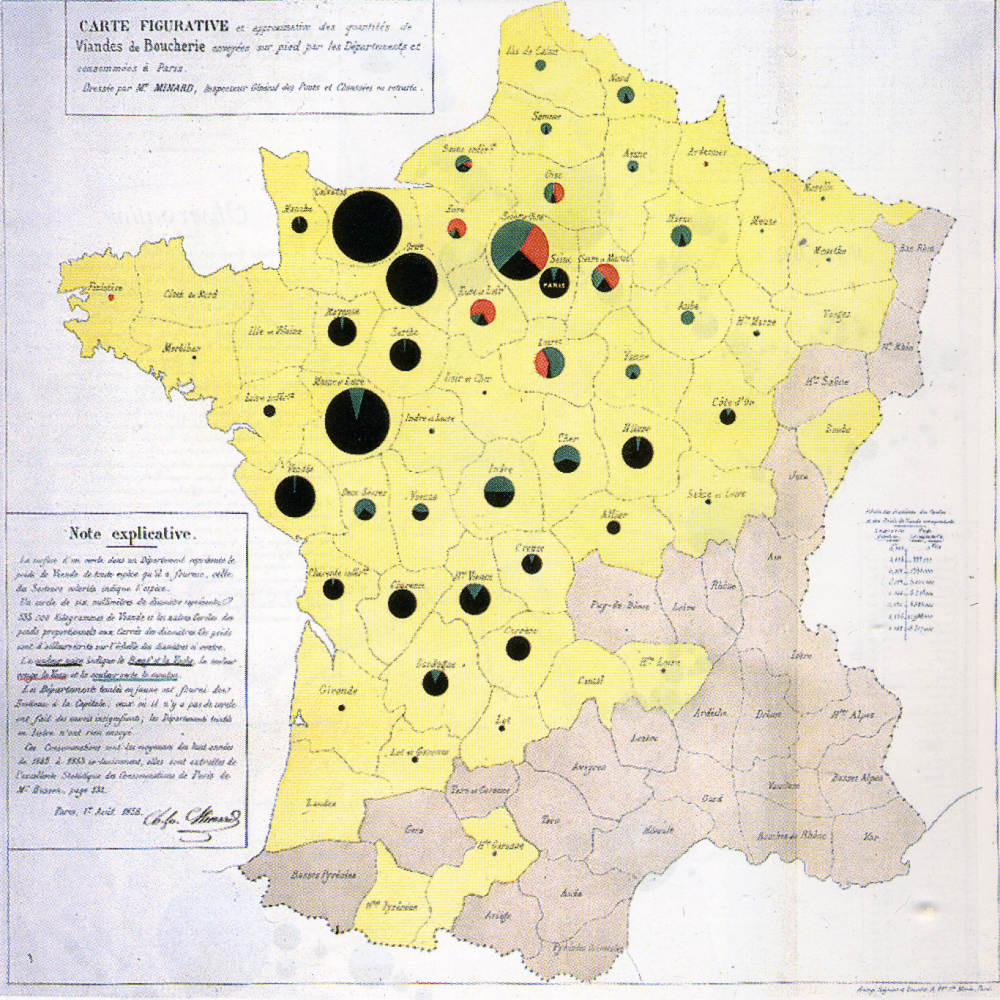
\includegraphics[width=0.4\textwidth,keepaspectratio]{images/history/minard.png}
\caption[
    A map using pie charts to represent the cattle sent from all around France for consumption in Paris., Urldate: 07.2016 \newline
\small\texttt{\url{https://upload.wikimedia.org/wikipedia/commons/1/1c/Minard-carte-viande-1858.png}}
]{A map using pie charts to represent the cattle sent from all around France for consumption in Paris.}
\label{fig:first-mixture}
\end{figure}

Another well known example of graphical representation from that century is the so called "cholera map" (see figure \ref{fig:cholera-map} on page \pageref{fig:cholera-map}.). Here, a dot map is used to display epidemiological data. This map could be used for knowledge creation in terms of the discovery of the source of a cholera epidemic.

\begin{figure}[!htb]
\centering
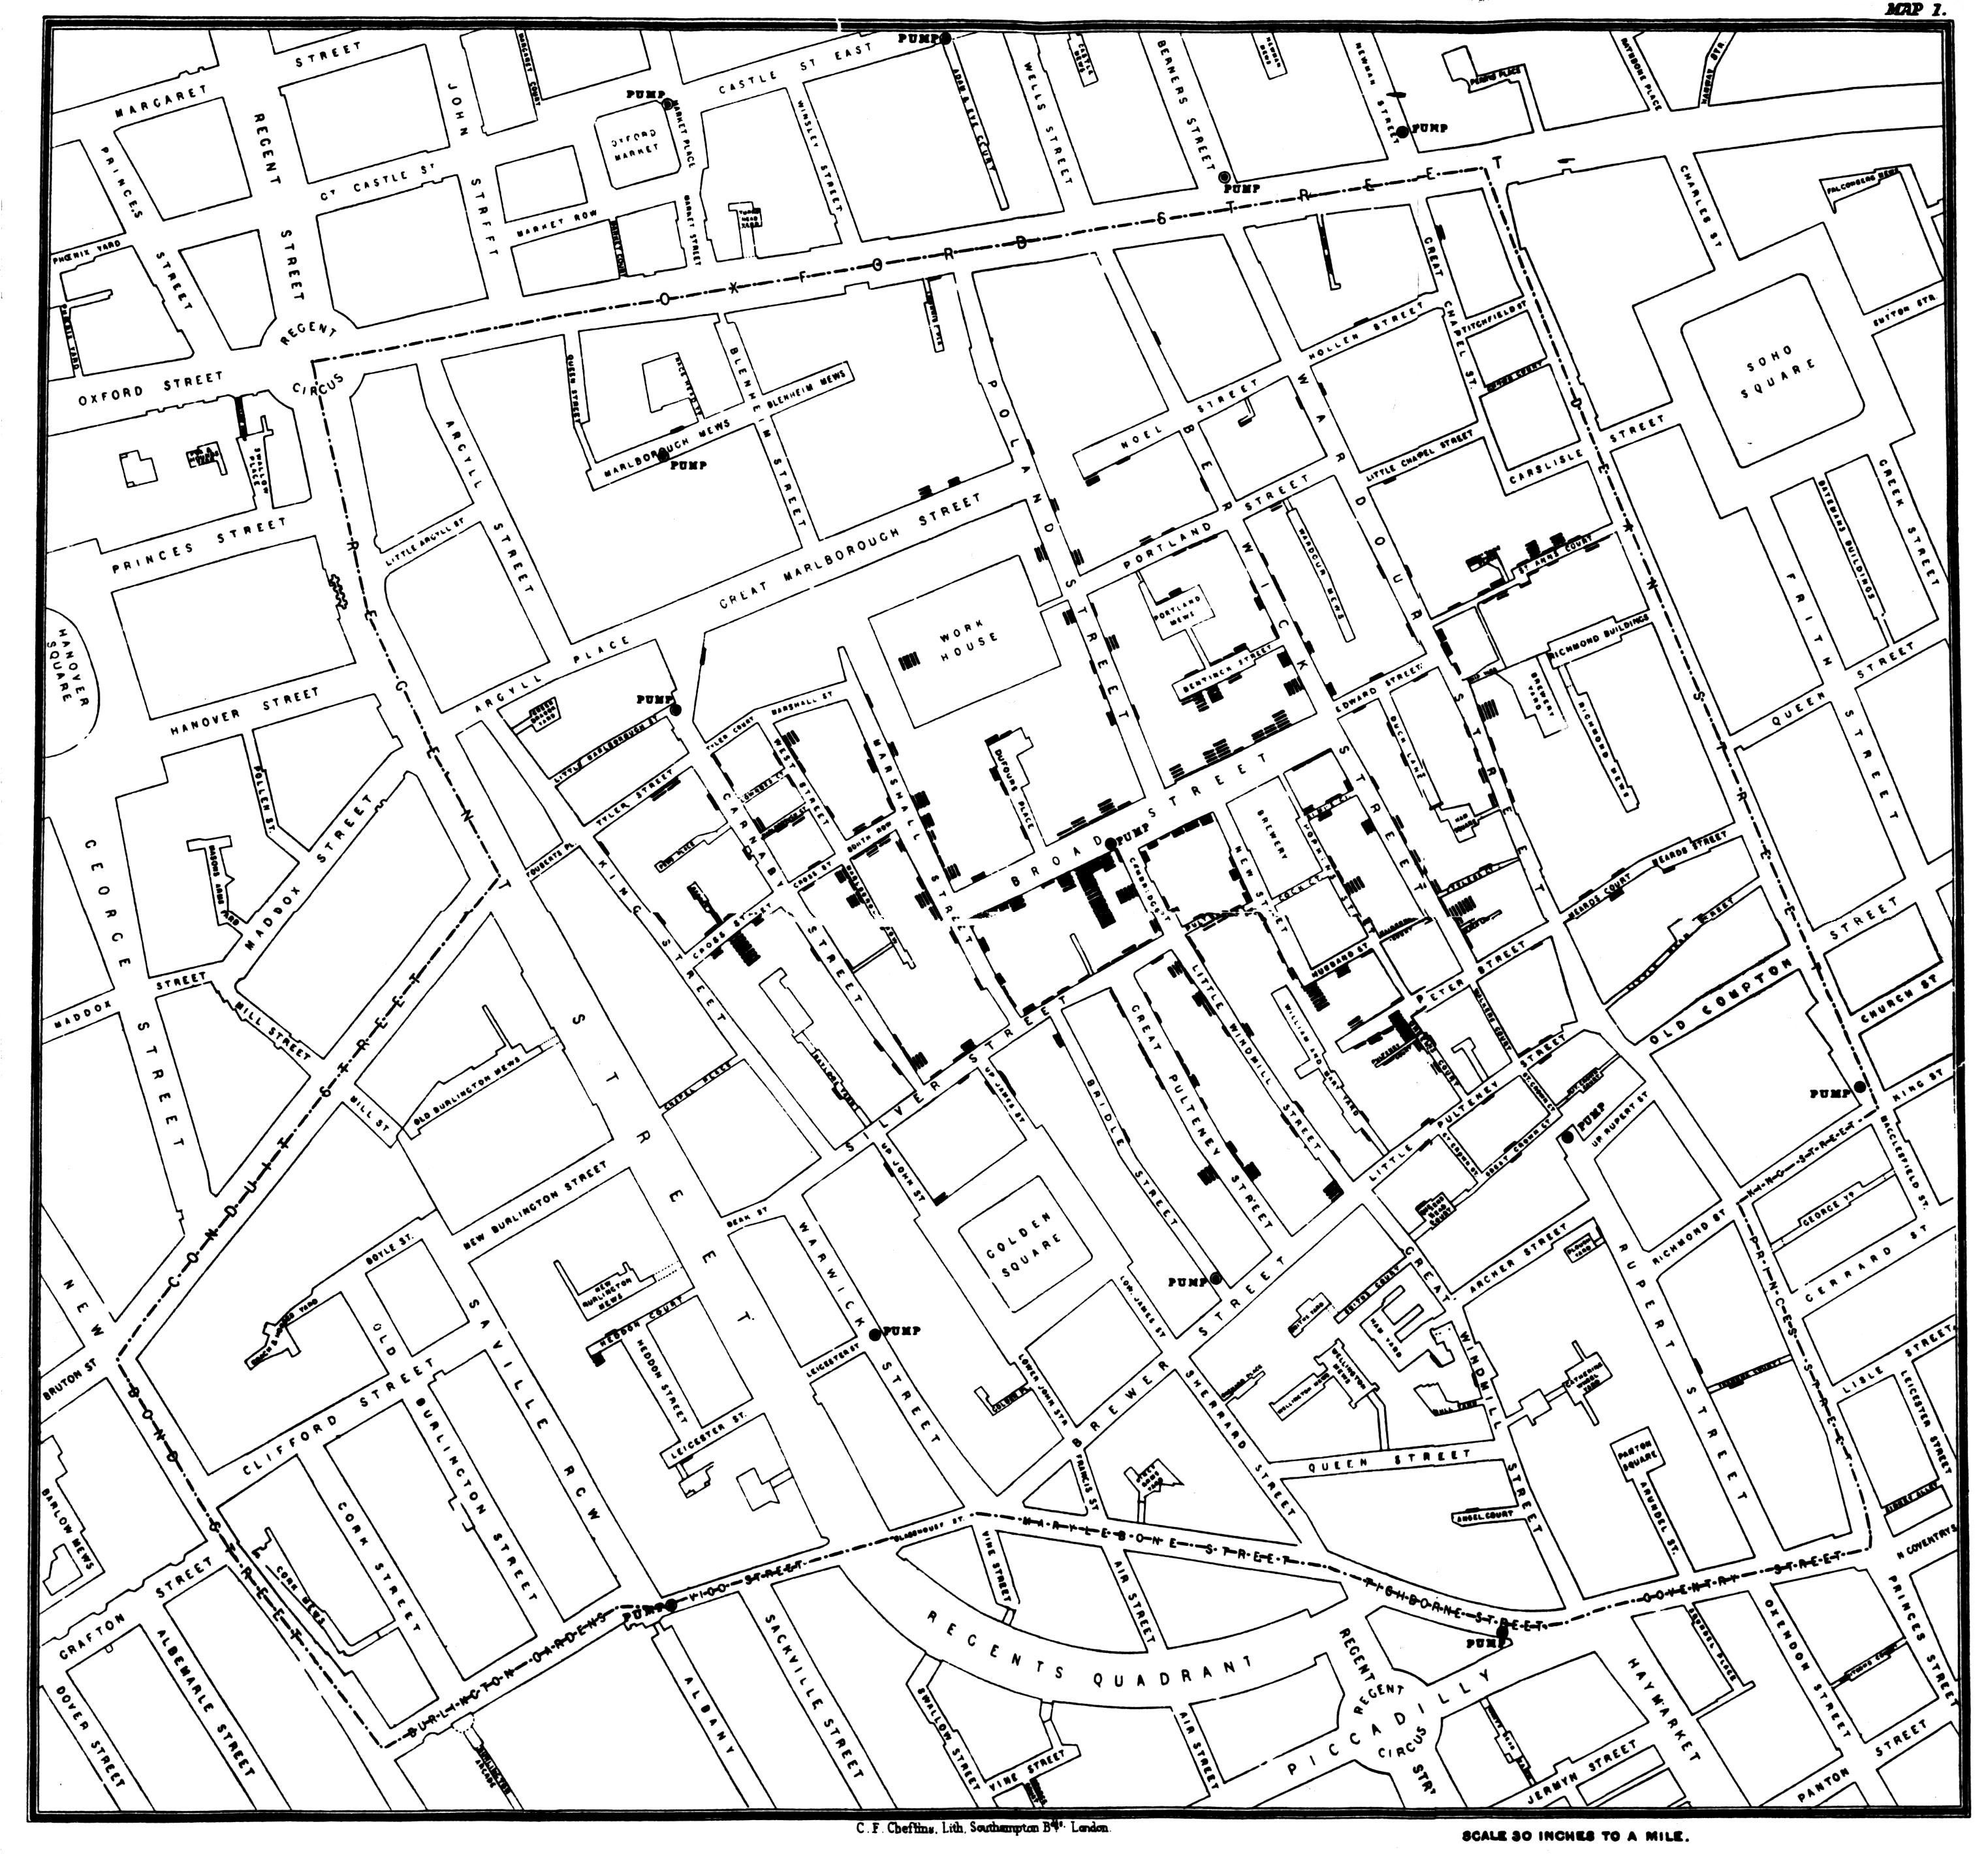
\includegraphics[width=0.8\textwidth,keepaspectratio]{images/history/cholera.jpg}
\caption[
    Dot map showing the clusters of cholera cases in the London epidemic of 1854., Urldate: 07.2016 \newline
\small\texttt{\url{https://upload.wikimedia.org/wikipedia/commons/2/27/Snow-cholera-map-1.jpg}}
]{Dot map showing the clusters of cholera cases in the London epidemic of 1854.}
\label{fig:cholera-map}
\end{figure}

In 1861, a new channel appeared in map based visualizations. It represents a weather map with glyphs (as a new channel) where each glyph embodies air pressure and barometric changes by means. Figure \ref{fig:weather-map} on page \pageref{fig:weather-map} shows the mentioned weather map.

\begin{figure}[!htb]
\centering
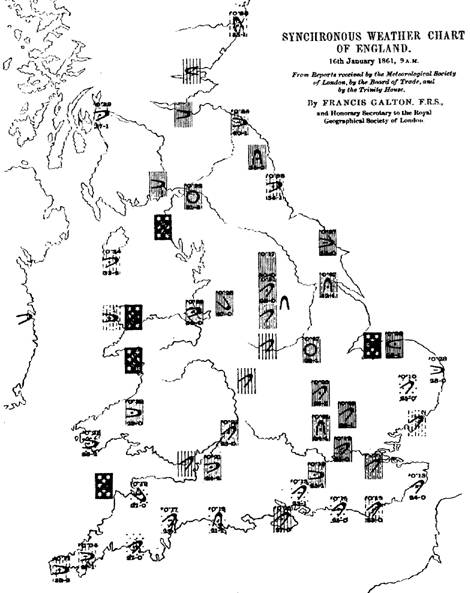
\includegraphics[width=0.4\textwidth,keepaspectratio]{images/history/weather.jpg}
\caption[
    A chart showing area of similar air pressure and barometric changes by means of glyphs displayed on a map., Urldate: 07.2016 \newline
\small\texttt{\url{http://datavis.ca/milestones//admin/uploads/images/galton-weather-charts2.gif}}
]{A chart showing area of similar air pressure and barometric changes by means of glyphs displayed on a map.}
\label{fig:weather-map}
\end{figure}

8 years later, Napoleon's march on Moscow (also called "the best graph ever produced") was visualized by Minard and is shown in figure \ref{fig:minard2} on page \pageref{fig:minard2}. Overall this figurative map can be described as the "Map of the successive losses in men of the French Army in the Russian campaign 1812-1813". The reason why this graph is sometimes referred to as the best graph ever produced is, because it contains multiple visual channels without influencing the comprehensibility of the graph. The following list describes some of the values encoded in the graph:
\begin{itemize}
\item The amount of men alive is encoded by the thickness of the colored lines in a rate of one millimeter for 10.000 men. The exact amount of men alive is also written beside the zones.
\item The color of the lines indicates the moving direction of the troops. Brown designates men moving into Russia and black are those on retreat.
\item The temperature is plotted at different points along the retreat at the bottom.
\end{itemize}
All in all, figure \ref{fig:minard2} on page \pageref{fig:minard2} encodes six different types of data in two dimensions:
\begin{enumerate*}
\item the number of Napoleon's troops,
\item the distance traveled
\item temperature
\item latitude and longitude
\item direction of travel
\item location relative to specific dates.
\end{enumerate*}
As of today, such a visual representation is known as a Sankey diagram which is a specific type of a flow diagram.

\begin{figure}[!htb]
\centering
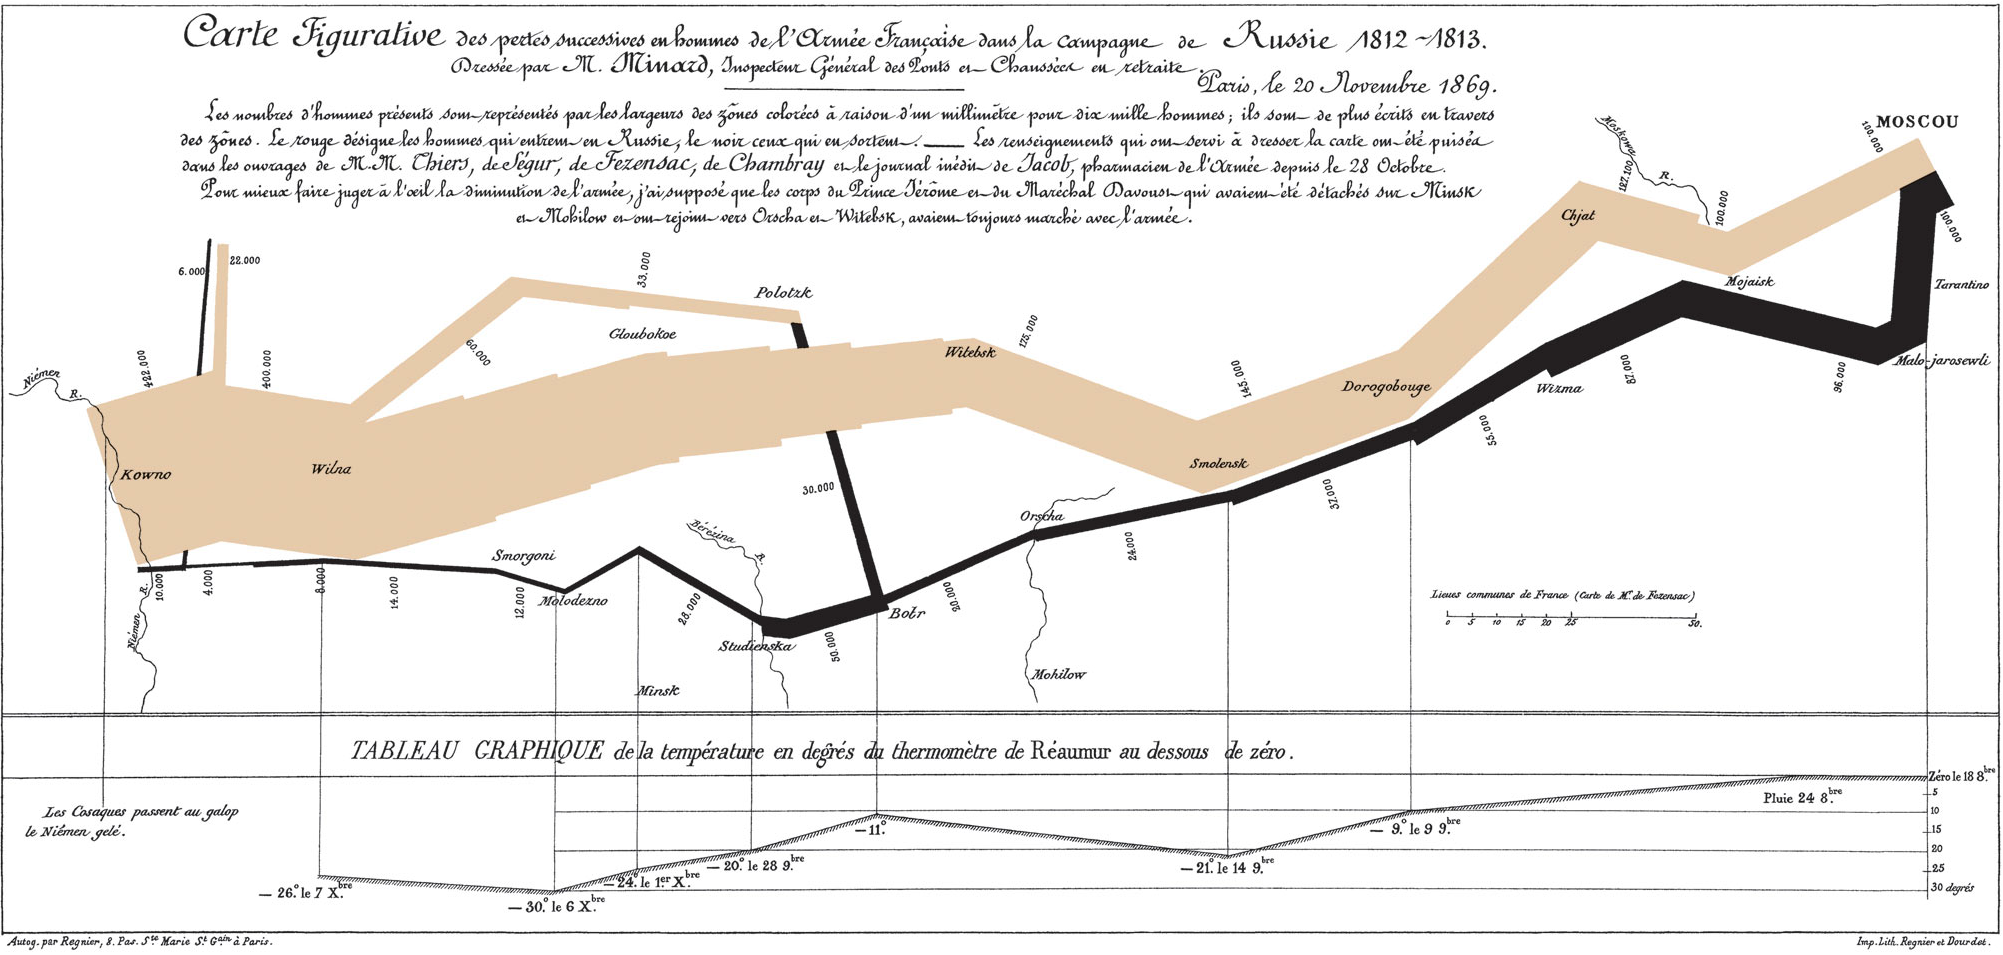
\includegraphics[width=0.8\textwidth,keepaspectratio]{images/history/minard2.png}
\caption[
    Charles Minard's map of Napoleon's disastrous Russian campaign of 1812., Urldate: 07.2016 \newline
\small\texttt{\url{https://upload.wikimedia.org/wikipedia/commons/2/29/Minard.png}}
]{Charles Minard's map of Napoleon's disastrous Russian campaign of 1812.}
\label{fig:minard2}
\end{figure}

If the literature refers to the 19\textsuperscript{th} century as "the golden age", they also often refer to the first half of the 20\textsuperscript{th} century as the "modern dark ages" of visualization. Only a few graphical innovations arised because in this period statistical graphics became to be common practice. Nonetheless, visual representations were used to provide new insights, discoveries and theories in this period. This was probably the first time graphical methods were used in different research fields such as astronomy, physics, and other sciences to justify hypotheses. Another research, which had a lot of impact in the research field of data visualization, was about comparisons of the efficacy of various graphic forms. In the mid 1960s, three developments made a significant impact on data visualizations:
\begin{enumerate}
\item \ac{EDA} was first mentioned by John W. Tukey in a paper called "The Future of Data Analysis". He demanded a strict distinction between data analysis as a legitimate branch of statistics and mathematical statistics.
\item The book called "Sémiologie graphique" (Semiology of graphics) was written and published by Jacques Bertin. To some
\begin{quote}
"this appeared to do for graphics what Mendeleev had done for the organization of the chemical elements, that is, to organize the visual and perceptual elements of graphics according to the features and relations in data."
\end{quote}
\item Computer processing of data arised, which offered more flexibility and possibilities in constructing graphic forms by programs.
\end{enumerate}

By the end of the 20\textsuperscript{th} century new research fields emerged and significant intersections and collaborations began: computer science research combined with the developments in data analysis provided new paradigms, languages and helpful packages in order to create statistical and data graphics. Thus a tremendous growth in new visualization methods and techniques appeared anew.
Another important innovation in that period were new paradigms  concerning direct manipulation of data (linking, brushing, selction, focus, etc. (for a detailed explanation see chapter \ref{s:basics} on page \pageref{s:basics}.)).

\subsubsection{Definition}
\label{s:definition}
\cbstart
The main goal of this Section is giving an overview of the definitions in literature of the term \textit{visualisation}. The first definitions appeared are taken from the beginnings of the research field of visualisation. The latter ones bear a reference to the technology available nowadays.
\cbend
Visualisation is first mentioned but not defined in 1953 in cartographic literature, in an article by University of Chicago geographer Allen K. Philbrick. \citeauthor{mccormick:1987} took up the term and defined it as follows:
\begin{quote}
 "Visualisation is a method of computing. It transforms the symbolic into the geometric, enabling researchers to observe their simulations and computations. visualisation offers a method for seeing the unseen. It enriches the process of scientific discovery and fosters profound and unexpected insights. In many fields, it is already revolutionizing the way scientists do science.

 Visualisation embraces both image understanding and image synthesis. That is, visualisation is a tool for both for interpreting image data fed into a computer, and for generating images from complex multi-dimensional data sets. It studies those mechanisms in humans and computers which allow them in concert to preceive, use and communicate visual information \iacite{mccormick:1987}."
\end{quote}

In 1987, new developments in the field of computer science prompted the National Science Foundation to redefine the term. The report of the redefinition placed visualisation at the convergence of computer graphics, image processing, computer vision, computer-aided design, signal processing, and user interface studies \iacite{mccormick:1987}. \citeauthor{Phillips2010} discuss three elemental issues existing today in the research field of visualisation:

\begin{enumerate}
\item to settle on a definition for the term \textit{visualisation}
\item to clarify the underlying presumptions and
\item to decide how to document both short-term and long-term effectiveness.
\end{enumerate}

\begin{quote}
The status of terms, often used interchangeably, such as \textit{visualisation}, \textit{visual representation}, \textit{visual media}, \textit{media literacy}, \textit{visual communication skills}, \textit{visual literacy}, \textit{illustrations}, and \textit{media illustrations}, is yet to be clarified. Furthermore, the routine confusion between pictures or visual images and reality is a fundamental and persistent problem \iacite{Phillips2010}.
\end{quote}

Because of the wide reach of the term, \citeauthor{Phillips2010} use a series of five steps in order to tell how \textit{visualisation} is defined in literature. The steps can be summarized as follows:
\begin{enumerate}
\item A search of all relevant sources, the identification of vocabulary and the mapping of the citations.
\item Classify the types of research into explanatory, exploratory, descriptive studies and ``other''.
\item Analyse and evaluate the assertions made in step two.
\item Organization of the reviews through comparisons of the literature, in order to identify areas of difference and similarity.
\item Mapping the collected information on several categories.
\end{enumerate}
The evaluation of this method used a total of 247 articles, ranging from the year 1936 to 2009. Out of those articles, 56\% were empirical studies and 44\% discussion articles. \citeauthor{Phillips2010} found out, that the attempt to define \textit{visualisation} in literature is not possible. The term is frequently substituted with terms like \textit{visual aid}, \textit{image}, \textit{visual literacy} etc.

To clarify the term with a relation to the progress made the last years, two well known online dictionaries are used. One possible generic definition could be the one from Oxford Dictionaries\footnote{See \href{https://www.oxforddictionaries.com/definition/english/visualisation}{https://www.oxforddictionaries.com/definition/english/visualisation}}:

\begin{quote}
\begin{enumerate}
\item ``The representation of an object, situation, or set of information as a chart or other image.''
\item ``The formation of a mental image of something.''
\end{enumerate}
\end{quote}

Even though the noun \textit{visualisation} has a very close related verb, \citeauthor{Phillips2010} noted the important distinction between those. The noun ``[\ldots] directs the attention to the product, the object, the 'what' of visualisation, the visual images. The verb of visualisation, on the other hand, makes one attend to the process, the activity, the skill, the 'how' of visualizing.''\iacite{Phillips2010}.

% TODO: check what to do when table is removed
Another possible generic definition for \textit{visualisation} is taken from the Merriam Webster Online Dictionary\footnote{See \href{http://www.merriam-webster.com/dictionary/visualization}{http://www.merriam-webster.com/dictionary/visualization}}. It is close to the one taken from the Oxford Dictionaries but has one significant distinction: ``The act or process of interperting in visual terms or of putting into visible form''. Compared to the statements of \citeauthor{Phillips2010}, this dictionary does not distinguish the process and the act of \textit{visualisation}.

However, combining the already mentioned definitions of terms with the research results from \citeauthor{Phillips2010}, a three-fold distinction of definitions is visible:
\begin{enumerate}
\item Physical objects serving as visualisations (e.g. geometrical illustrations). These objects are viewed and interpreted by a person for the purpose of understanding something.
\item Mental objects pictured in the mind (e.g. mental imagery). These are imaginative constructions of some possible visual experiences.
\item Cognitive processing in which visualisations are interpreted, either physical or mental (e.g. cognitive manipulation of visual representations by the mind). This often refers to an act of deriving meaning from a physical or mental object.
\end{enumerate}

\cbstart
\citeauthor{Munzner2014} takes the available technology into account and therefore provides a more advanced definition. She combines the term \textit{visualisations} with computer-based systems yielding new definition possibilities to the whole term. Nonetheless, she does not revoke the older definitions and defines the term on the basis of them.
Using computer-based systems help people to carry out tasks more effectively.
\textit{Visualisations} created by systems cannot replace a human with computational decision-making methods, they are needed when there is a need to augment human capabilities. Furthermore, besides taking the process of creation into account, \textit{visualisations} also need to consider interaction with visual representations \iacite{Munzner2014}.

According to \citeauthor{Phillips2010} the distinction between physical and mental visualisation objects are obvious. This statement is also verified by the given definition of \citeauthor{mccormick:1987} where this exact distinction is already made. However the distinction between the visualisation itself and the thinking involved in interpreting it is also important \iacite{Phillips2010}. \citeauthor{Munzner2014} extends the term of \textit{visualisation} with the combination of computer-based systems and the thereby existing possibilities of interaction yielding a much broader term with three more limitations:
\begin{enumerate*}[label={(\arabic*)}]
\item the limitations of computers,
\item of humans,
\item and of displays \iacite{Munzner2014}.
\end{enumerate*}

\cbend

\subsubsection{Varieties of visualisations}
\label{s:definitions-types}
\cbstart
In order to fully understand this Section, the definition of the term \textit{visualisation} needs to be clear (see Chapter \ref{s:definition} on page \pageref{s:definition} for more information).

So far the term of visualisation has been defined. Formerly, the research field of visualisation was built upon two major parts: the field of \ac{InfoVis} and the one of \ac{SciVis}. The following list briefly describes each field. However, the distinction between those fields becomes more and more blurred. This is due to the fact that the data used in visualisations are not necessarily of a single nature, e.g. geo-spatial data only. With today's possibilities in data acquisition and preprocessing, there are no limitations in combining data from different natures.

\begin{description}

\item[\acl{InfoVis}] \hfill \\
\citeauthor{Friendly.2001} refered to \ac{InfoVis} to the broadest term that could be used to group all the developments mentioned in Section \ref{s:history}. From a very basic point of view, almost everything, if sufficiently organised, contains information in some kind. Therefore the term could be used for the earliest attempts to scratch information on rocks and to the earliest use of diagrams in history \iacite{Friendly.2001}.

\citeauthor{Ferreira2003} had a more contemporary definition of \ac{InfoVis}. They said the graphical models may represent abstract concepts and relationships that do not necessarily have a counterpart in the physical world. An example of the mentioned relationship would be an information describing user accesses to pages of an internet portal. It is typical for each data unit to describe multiple related attributes (usually more than four) that are not of some kind of spatial or temporal nature. Although spatial and temporal attributes may occur, the data existed in an abstract data space \iacite{Ferreira2003}.
\newpage
\item[\acl{SciVis}] \hfill \\
A close related, yet distinct field, called \ac{SciVis}, was primarily concerned with the visualisation of 3D phenomena, where the emphasis was on realistic renderings of volumes, surfaces, etc. 3D Phenomena for \ac{SciVis} could be of architectural, meteorological, medical nature and so forth \iacite{Friendly.2001}.

\citeauthor{Ferreira2003} also had a similar definition for \ac{SciVis}. They defined the term as the graphical models which are typically constructed from measured or simulated data representing objects or concepts associated with phenomena from the physical world. As such, the derived visualisations represented objects that exist in a 1D, 2D or 3D object space. The presence of spatial and temporal dimensions could be included in the data and thus are determinants in deriving visual representations from it \iacite{Ferreira2003}.
\end{description}

In the early 1980s, a french graphic theorist named Jacques Bertin set a milestone in the area of scientific research, as already mentioned in Chapter \ref{s:history} on page \pageref{crossref:bertain}. Based on his work, the semiology of graphics, the research field called \ac{GeoVis} arose. His work shows a strong focus in the research of the potential for the use of dynamic visual displays as prompts for scientific insight and of the methods through which dynamic visual displays might leverage perceptual cognitive processes to facilitate scientific thinking \iacite{maceachren:2004}.

The broad term \ac{GeoVis} has the same problems as the other one concerning a specific definition: the term is used in many different research fields. Thus, multiple definitions suitable for the particular case exist in literature. This thesis gives an overview of some definitions, which also apply to the use of the term in this thesis.
The following definition according to the 2001 research agenda of \ac{ICA}, Commission on visualisation and Virtual Environments, is most widely accepted:
\begin{quote}
``Geovisualisation integrates approaches from visualisation in scientific computing, cartography, image analysis, information visualisation, exploratory data analysis and geographic information systems to provide theory, methods, and tools for visual exploration, analysis, synthesis, and presentation of geospatial data \iacite{Longley2005}.''
\end{quote}

\citeauthor{Noellenburg2007} mentions other definitions which have a more human-centred view and describe geovisualisation as
\begin{quote}
``[\ldots] the creation and use of visual representations to facilitate thinking, understanding, and knowledge construction about geospatial data'', or as ``the use of visual geospatial to display and to explore data and through that exploration to generate hypotheses, develop problem solutions and construct knowledge \iacite{Noellenburg2007}.''
\end{quote}

\newpage
Even though the definitions are slightly constrasting, they share one thought: \ac{GeoVis} is a multidisciplinary task and since it is a human being using those visualisations to explore data and construct knowledge, \ac{GeoVis} takes the user needs into account above everything else.

\cbend

\subsubsection{Why, when and how to visualise}
\label{s:basics}
\citeauthor{Munzner2014} answers many questions concerning the usage of visualisations in her book called ``Visualization Analysis and Design'' \iacite{Munzner2014}. This Chapter discusses the most important answers because they are a necessity in understanding the questions of when, why and how to visualise. Furthermore, it introduces an analysis framework for visualisation tools in order to
put different tools in comparison.

From today's perspective with the ability to use artificial intelligence and machine learning, the question if we still need a human in order to create visualisations is valid. This question has a simple answer: if well-defined questions to ask about data exist in advance, it is possible to answer these purely with computational techniques from fields such as statistics and machine learning. If a solution to a problem has been fully automatised and has been deemed to be acceptable, there is no need for human judgement anymore and thus no need to design a visualisation tool. An example of a practical application would be the domain of stock market trading. A tool in that field can be fully automatised. There are currently many deployed systems for high-frequency trading. Those systems make decisions about buying and selling stocks when certain market conditions hold \iacite{Munzner2014}. Some other reasons where computers beat humans are mentioned below:
\begin{itemize}
\item Scale: Drawing a dataset of hundreds of thousands of items by hand is infeasible and would take a lot of time.
\item Efficiency: Once a problem has been solved with a computer it can be reused  indefinitely for different datasets and scenarios.
\item Quality: Precise data-driven rendering.
\end{itemize}
However, many analysis problems are poorly specified. Either the approach to the problem is unknown, or it is not obvious which questions the data could or should answer. In such a case, \citeauthor{Munzner2014} says, that the best path forward is an analysis process with a human in the loop \iacite{Munzner2014}. Even though there are a lot of use cases for a human in the loop, this paper only discusses one which deals with \ac{EDA} (see Chapter \ref{s:eda} on page \pageref{s:eda} for more information.), which is essential for this thesis. Exploratory analysis in scientific discovery is a common case of the need of a human. A long-term visualisation tool which could be developed is a tool with the goal of speeding up and improving user's ability to generate and check hypotheses \iacite{Munzner2014}.

% Maybe use ability matrix here

Another important question answered by \citeauthor{Munzner2014} is: why depend on vision? As Chapter \ref{s:definition} on page \pageref{s:definition} already mentions, a part of visualisation is based on exploiting the human visual system as a means of communication. A significant amount of visual information processing occurs in parallel through high-bandwidth channels to our brain. One example \citeauthor{Munzner2014} mentions is visual popout: one red item in a sea of gray ones is immediately noticed. This exploit of a human visual system can be used effectively to highlight specific information and to draw attention to a part of the visualisation.

Furthermore a single static view can show only one aspect of a dataset. This fact is already part of the answer of the next question: why use interactivity? Even though there are combinations of simple datasets and tasks where only a single visual encoding and therefore a single static view is needed, it does not apply for large complex datasets where interactivity allows to change displays and supports many possible queries. Interactivity could be used to investigate multiple levels of detail at once, ranging from a very specific detailed view of a small part to a very high-level summarisation \iacite{Munzner2014}.

The main goal of a design of a visualisation is to satisfy rather than optimise. One of the many possible good solutions to a problem is much harder to find than one of the even larger number of bad ones. Yet the validation of satisfaction is very difficult because there are so many questions considering wheter a visualisation tool has met the design goals \iacite{Munzner2014}.

Furthermore considering at least three different kinds of limitations when designing or analysing visualisations is important:
\begin{enumerate}
\item computational capacity
\item human perceptual and cognitive capacity
\item display capacity
\end{enumerate}

All three limitations can be subsumed with the term scalability.

One of the most important questions \citeauthor{Munzner2014} answers is called: why analyse? In order to answer the question, she features an analysis framework that helps to think about design choices for visualisations systematically. Figure \ref{fig:an-framework} on page \pageref{fig:an-framework} shows the high-level framework she provides for analysing a visualisation's use according to three questions: what data does a user see, why does the user intend to use a visualisation tool and how are the visual encoding and interaction idioms constructed in terms of design choices \iacite{Munzner2014}.

\begin{figure}[!htb]
\centering
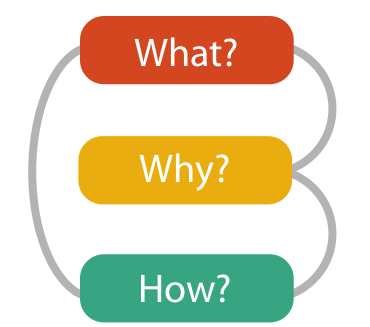
\includegraphics[width=0.3\textwidth,keepaspectratio]{images/basics/analysis-framework.png}
\caption[
    Three-part analysis framework for a visualisation instance: why is the task being performed, what data is shown in the views, and how is the visualisation idiom constructed in terms of design choices \iacite{Munzner2014}.
]{Three-part analysis framework for a visualisation instance: why is the task being performed, what data is shown in the views, and how is the visualisation idiom constructed in terms of design choices.}
\label{fig:an-framework}
\end{figure}

At this time, two out of three main questions for this chapter have been solved. A visualisation should be made if there are no questions according to given data known in advance. If a visualisation is combined with \ac{EDA}, it emphasises knowledge construction over knowledge storage or information transmission, therefore answering the question why to visualise.

In order to answer the last main question of this section, \citeauthor{Munzner2014} features Figure \ref{fig:how} on page \pageref{fig:how} which provides a preview of a set of design choices, with a high-level breakdown into four major classes:

\begin{enumerate}

\ditem{Encode} \hfill \\
This first part of the figure deals with the encoding of how to arrange data spatially and shows five different choices:
    \begin{enumerate*}[label={(\arabic*)}]
    \item express values,
    \item separate,
    \item order and
    \item align regions and
    \item use given spatial data directly.
    \end{enumerate*}
Another important aspect this part features is the usage of nonspatial visual channels including color, size, angle, shape and so forth according to the type of attribute. These channels are explained in detail later in this chapter.

\ditem{Manipulate} \hfill \\
The second part handles different approaches manipulating different aspects of the visualisation like changing any aspect of the view, selecting elements from within the view and navigating to change the viewpoint within the view.

\ditem{Facet} \hfill \\
The third part shows three different choices of how to facet data between views.

\ditem{Reduce} \hfill \\
The fourth part again mentions three different options for how to reduce the data shown.

\end{enumerate}

\begin{figure}[!hbt]
\centering
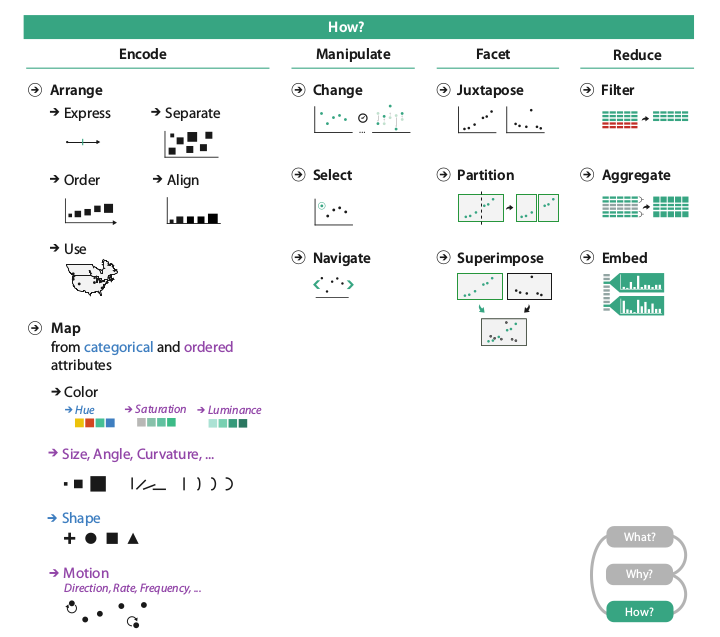
\includegraphics[height=10cm,keepaspectratio]{images/basics/how.png}
\caption[
    How to design visualisation idioms: encode, manipulate, facet, and reduce \iacite{Munzner2014}.
]{How to design visualisation idioms: encode, manipulate, facet, and reduce.}
\label{fig:how}
\end{figure}

Even though the main questions of this section have been answered, one more question appeared in combination with the analysis framework: what? To summarise the usage of this framework, two more figures are introduced: Figure \ref{fig:what} and \ref{fig:why} on page \pageref{fig:what} and \pageref{fig:why}.

\cbstart
Figure \ref{fig:what} starts with differentiating five different types of data (items, attributes, links, positions and grids) which is followed by dataset types consisting of different combinations of these data types. Considering a flat table as an example, the terms used in this thesis are the same as the ones \citeauthor{Munzner2014} uses. A row in the table represents an item of the data, whereas each column is an attribute of an item \iacite{Munzner2014}.
\cbend
The availability of these datasets can be either immediately in the form of a static file, or in the form of a data stream.

\begin{figure}[!htb]
\centering
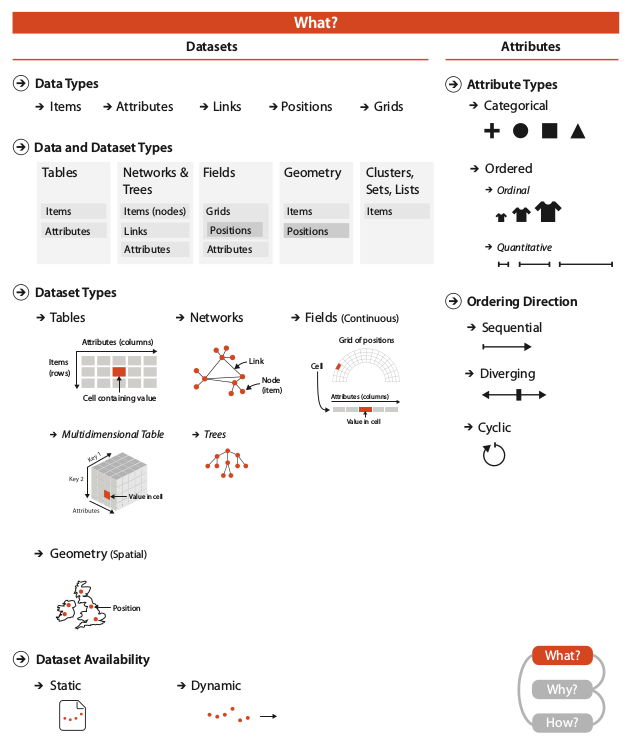
\includegraphics[height=10cm,keepaspectratio]{images/basics/what.png}
\caption[
    What can be visualised: data, datasets, and attributes \iacite{Munzner2014}.
]{What can be visualised: data, datasets, and attributes.}
\label{fig:what}
\end{figure}

Figure \ref{fig:why} is shown for the sake of completeness in combination with the analysis framework. It features two main parts: the reasons why a visualisation tool is being used (actions and targets). The highest-level actions to use visualisations are either to consume or produce information. The second-level action can be summarised as a search. From an abstract point of view, there is no difference in knowing the target or location a user is looking for or not. It ends up with either looking up that specific target or browsing and exploring the given visualisation in order to find it. At the low level, queries can be divided into three parts: identification of a specific target, comparison of multiple targets and the summarisation of all targets.
The targets for all kinds of data are finding trends and outliers. This can be divided into two parts:
\begin{enumerate*}[label={(\arabic*)}]
\item finding one value, the extreme values or the distribution of all values for exactly one attribute, or
\item finding dependencies, correlations or similarities between multiple attributes.
\end{enumerate*}

\begin{figure}[!htb]
\centering
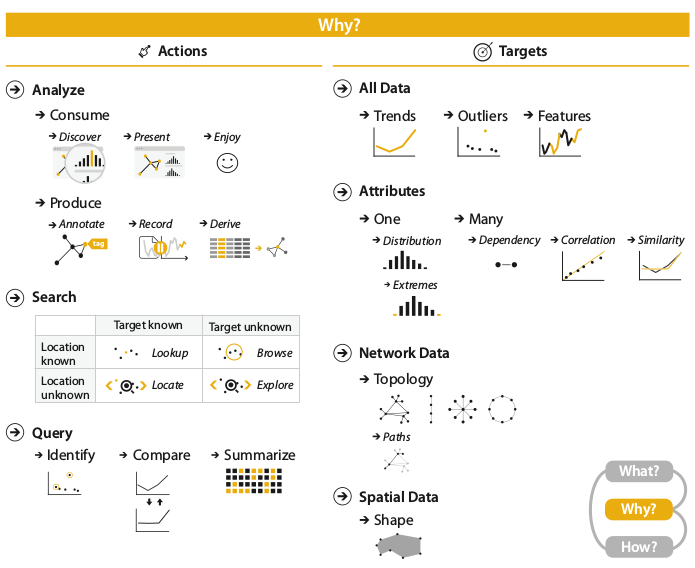
\includegraphics[height=7.5cm,keepaspectratio]{images/basics/why.png}
\caption[
    Why people are using visualisations in terms of actions and targets \iacite{Munzner2014}.
]{Why people are using visualisations in terms of actions and targets.}
\label{fig:why}
\end{figure}

The discussed framework will be used as a basis to analyse the related work mentioned in this thesis.



% TODO: visualisations for presentation only; write something about this
\subsubsection{Exploratory data analysis}
\label{s:eda}
\citeauthor{Tukey1977} introduced and promoted the term of \ac{EDA} in 1977 to encourage statisticians to explore data and possibly formulate hypotheses that could lead to new data collection and experiments. Many \ac{EDA} ideas can be traced back to earlier authors but \citeauthor{Tukey1977} summarized all of those idea with the introduced term. Even though the earlier ideas have all been in combination with statistics, \citeauthor{Tukey1977} encouraged the research field of statistics to use the capabilities of dynamic visualizations in combination with given data. Before that encouragement, statisticians had a strong focus on statistical hypothesis testing without any visualization. This development helped professional field to identify outliers, trends and patterns in data in a visual and understandable way \iacite{Tukey1977}. Thus it is possible to derive objectives of \ac{EDA} \iacite{Behrens1997}:

\begin{itemize}

\item Suggest hypotheses about the causes of observed phenomena.
\item Assess assumptions on which statistical inference will be based
\item Support the selection of appropriate statistical tools and techniques
\item Provide a basis for further data collection through surveys or experiments.

\end{itemize}

As of today, there are a number of techniques assisting the field of \ac{EDA}, but the field is more characterized by the attitude taken than by particular techniques \iacite{Tukey1980}. Typical graphical techniques used in \ac{EDA} are box plots, histograms, scatter plots, stem-and-leaf plots, and so forth. This chapter will only discuss histograms in detail.

\citeauthor{Pearson1895} introduced histograms as a graphical representation of the distribution of numerical data. It is an estimate of the probability distribution of a quantitative variable \iacite{Pearson1895}. As the history of visualization shows (see chapter \ref{s:history} on page \pageref{s:history} for more detail.), cartography also had the goal to visualize distributions on thematic maps. It emphasized especially a spatial variation of one or a small number of geographic distributions.

With this in mind, this chapter could be taken to subsume the two main focii of the thesis: statistical graphics and thematic cartography. Both of these are concerned with graphical representations of quantitative and categorical data, but driven by different representational goals. \citeauthor{Friendly.2001} describe the objectives of cartographic visualization as finding the representation constrained to a spatial domain whereas statistical graphics try to apply to any domain in the service of statistical analysis \iacite{Friendly.2001}. In addition, cartography and statistical graphics share the common goals of visual representation for exploration and discovery. These range from the simple mapping of locations (land mass, rivers, terrain), to spatial distributions of geographic characteristics (species, disease, ecosystems), to the wide variety of graphic methods used to portray patterns, trends, and indications \iacite{Friendly.2001}. The combination of analytical reasoning with visual representations lead to the research field of visual analytics.




\subsubsection{Visual analytics and visual design principles}
\label{s:va}
According to \citeauthor{Keim2010}, visual analytics "[\ldots] is not easy to define, due to its multi-disciplinary nature involving multiple processes and the wide variety of application areas \iacite{Keim2010}." Based on current practice, they define visual analytics as the combination of automated analysis techniques with interactive visualizations for an effective understanding, reasoning and decision making on the basis of very large and complex datasets \iacite{Keim2010}.

So, based on the definition, \citeauthor{Keim2010} elaborate the objectives of visual analytics to state that it is the creation of tools and techniques to enable people to:

\begin{itemize}
\item Summarize information and derive insight from heterogeneous and often conflicting data
\item Detect the expected and discover the unexpected
\item Provide reasonable and understandable evaluations
\item Communicate these evaluations effectively for action
\end{itemize}

The following part in this chapter gives an overview of how visual analytics tries to achieve these objectives to generate knowledge from data. Based upon the knowledge gathered in this chapter and the chapters before, it is possible to derive design principles for good visualizations.

Figure \ref{fig:va-process} on page \pageref{fig:va-process} shows an abstract overview of the visual analytics process. It contains different stages, represented as colored ovals, and their corresponding transitions, represented as arrows. The first step of the process deals with the integration of heterogeneous data sources. This integration includes tasks like data preprocessing, transforming, cleaning, normalization, grouping and fusion. All those tasks are indicated by the transformation transition onto the data oval. After the transformation, the analyst has two different options to choose \iacite{Keim2010}:

\begin{enumerate}
\ditem{Automated data analysis} \hfill \\
If an automated model was chosen first, data mining methods are applied to generate statistical models out of the original data. Once the model is made, the analyst only needs to refine its parameters and evaluate it afterwards. The advantage of this choice is the scalability because it can be fully automatized. This automatization is also the main disadvantage. The model runs in a black box fashion, ignoring all interactions. If this is done, the evaluation of the model can be accomplished with a visualization. This makes it possible to interact with the data later on \iacite{Keim2010}.

\ditem{Visual data exploration} \hfill \\
If visual data exploration is chosen first, interaction with the generated visualization is needed to construct insightful information. Interaction could be integrated by zooming or considering different views on the data. Findings can be used to create automatic models. The main advantage of this approach is the interaction with an analyst, thus offering more flexibility and possibilities. On the other hand, it is not scaleable in any way.
\end{enumerate}

\begin{figure}[!htb]
\centering
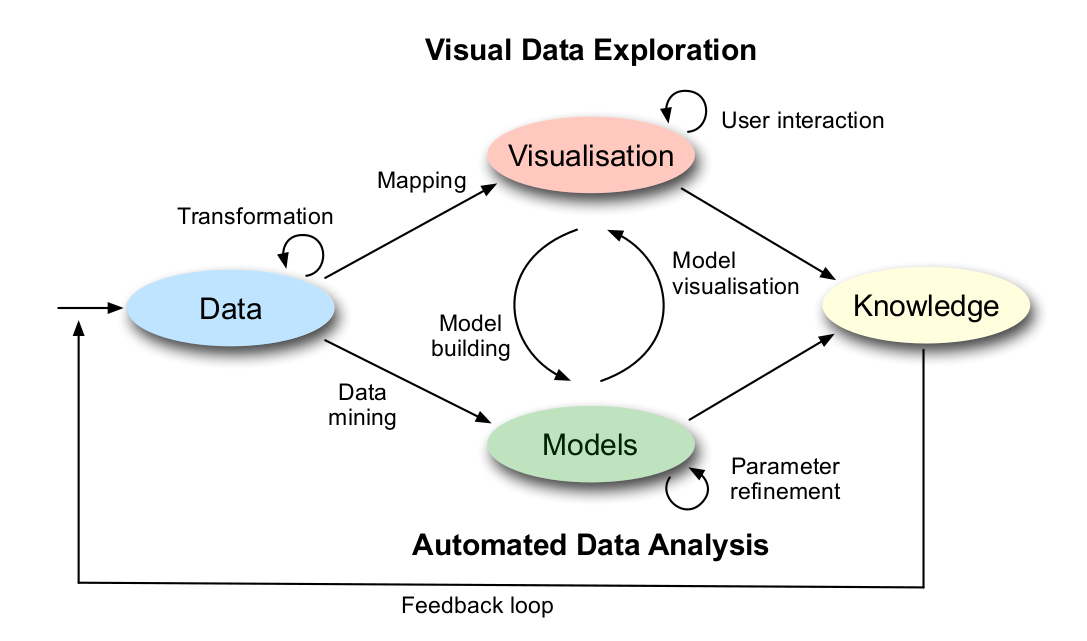
\includegraphics[height=5cm,keepaspectratio]{images/va/va-process.png}
\caption[
    The visual analytics process is characterised through interaction between data, visualisations, models about the data and the users in order to discover knowledge \iacite{Keim2010}.
]{The visual analytics process is characterised through interaction between data, visualisations, models about the data and the users in order to discover knowledge.}
\label{fig:va-process}
\end{figure}

If automated data and visual data analysis is used in an agile way like iterating both analysis methods in sequence until knowledge is discovered, misleading results in an intermediate step can be discovered and eliminated at an early stage and thus leading to higher confidence and better results \iacite{Keim2010}.

In summary, it can be said that the visual analytics process extracts knowledge gained from visualizations, automatized analysis and a human analyst combining these two.

Figure \ref{fig:va-related} on page \pageref{fig:va-related} shows the interdisciplinary character of visual analytics. With visualization as its core, other disciplines like data management, data analysis and data mining are close related and seem kind of obvious based on the knowledge of the visual analytics process and the definition of the term itself.

\begin{figure}[!htb]
\centering
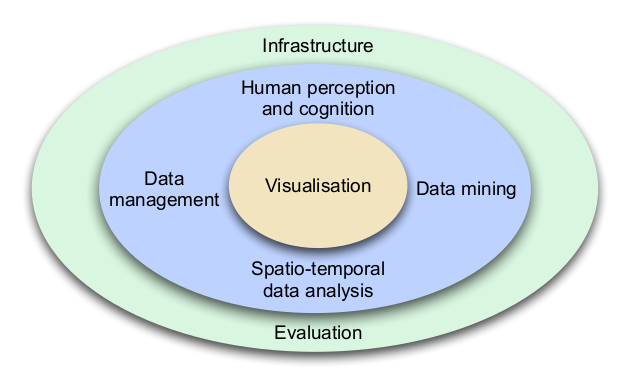
\includegraphics[height=5cm,keepaspectratio]{images/va/va-related.png}
\caption[
    Visual analytics with core adjacent disciplines \iacite{Keim2010}.
]{Visual analytics with core adjacent disciplines.}
\label{fig:va-related}
\end{figure}

In order to create visualization designs, it is needed to clarify the usage of marks and channels in designs first. Marks basically are geometric elements that depict items or links. Figure \ref{fig:va-marks} on page \pageref{fig:va-marks} shows examples of marks in different dimensions. Points count as a 0D mark, whereas lines belong to 1D marks, and areas to 2D marks. A visual channel controls the appearance of a given mark, independent of the dimensionality. Figure \ref{fig:va-channels} on page \pageref{fig:va-channels} shows a few channels that can encode information. The core of a design can be described as a combination of two aspects: graphical elements called marks, and visual channels.

\begin{figure}[!htb]
\centering
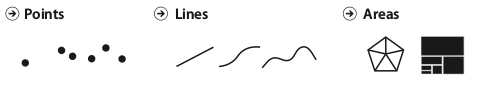
\includegraphics[width=0.5\textwidth,keepaspectratio]{images/va/marks.png}
\caption[
    Marks are geometric primitives \iacite{Munzner2014}.
]{Marks are geometric primitives.}
\label{fig:va-marks}
\end{figure}

\citeauthor{Munzner2014} states that all channels are not equal. She says using two different visual channels on the same data attribute results in different information after it has passed through the perceptual and cognitive processes of the human visual system. The usage of marks and channels in a design should be guided by the principles of expressiveness and effectiveness \iacite{Munzner2014}.

\begin{figure}[!htb]
\centering
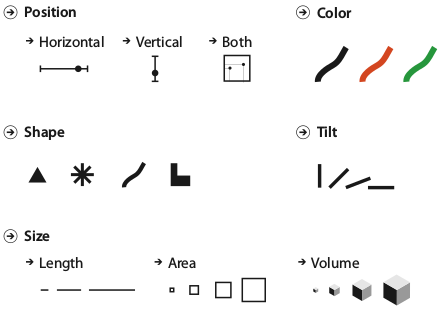
\includegraphics[height=5cm,keepaspectratio]{images/va/channels.png}
\caption[
    Visual channels control the appearance of marks \iacite{Munzner2014}.
]{Visual channels control the appearance of marks.}
\label{fig:va-channels}
\end{figure}

\begin{enumerate}
\ditem{The expressiveness principle} suggests that the used channel should express all of the information in the dataset attributes. The most fundamental expression of this principle is, that known pattern should be shown accordinly, e.g. sorted and ranked data should be shown in a way that this pattern is intrinsically sensed \iacite{Munzner2014}.

\ditem{The effectiveness principle} suggests that the importance of the data attribute should match the emphasis of the channel, so to say its noticeability \iacite{Munzner2014}.
\end{enumerate}

Figure \ref{fig:va-channels-ranked} on page \pageref{fig:va-channels-ranked} introduces visual channels ranked by their effectiveness. To fully understand this figure, it is first needed to explain different attribute types.

There are two major types: categorical and ordered. Within the ordered type, there is a distinction between ordinal and quantitative types. Categorical data attributes can be mathematically described as the attributes where only equality comparisons of attributes are possible ($=$, $\neq$). This does not exclude the usage of any arbitrary external ordering like alphabetically ordering because such orderings are not implicit in the attribute itself. However, ordered data allows the use of ranking in addition to equality comparisons because they have such an implication ($=$, $\neq$, $>$, $<$). As already mentioned, this type can be further subclassified. Quantitative data allow the usage of arithmetic operations because it is a measurement of magnitude. Only one furher distinction is needed to know if multiplication and division is possible or not. If the origin of the measurement is meaningful, like in length, mass, temperature, and so forth, it is possible to use the following arithmetic operations: $=$, $\neq$, $>$, $<$, $+$, $-$, $\times$, $\div$. If this is not the case, but the attribute still allows for zero arbitrary, the following arithmetic operations can be applied: $=$, $\neq$, $>$, $<$, $+$, $-$ \iacite{Stevens1946}.

\begin{figure}[!htb]
\centering
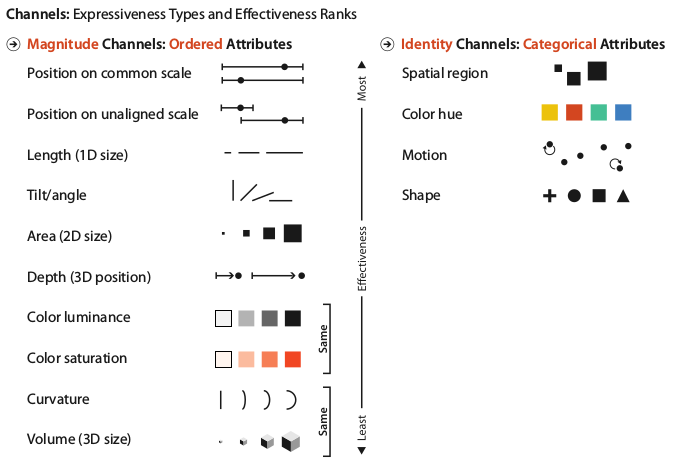
\includegraphics[height=10cm,keepaspectratio]{images/va/channels-ranked.png}
\caption[
    Channels ranked by effectiveness according to data and channel type. Ordered data should be shown with the magnitude channels, and categorical data with the identity channels \iacite{Munzner2014}.
]{Channels ranked by effectiveness according to data and channel type. Ordered data should be shown with the magnitude channels, and categorical data with the identity channels.}
\label{fig:va-channels-ranked}
\end{figure}

With the different attribute types defined and explained, the distinction and usage of magnitude and idendity channels, visible in figure \ref{fig:va-channels-ranked}, should be clear. The ranking ranges from the most effective channels at the top to the least effective ones at the bottom. The most effective visual channels for ordered attributes are based on spatial position, either aligned or unaligned. The next four channels (length, angle, area and depth) are somewhat combinable: length is a 1D size, whereas angle and area are used for 2D sizes and depth for 3D positioning. These channels are followed by two roughly equally effective ones: luminance and saturation, which in turn are followed by two channels roughly equal in terms of effectiveness: curvature and volume. The most effective idendity channel is spatial region, followed by color hue. In third position is the motion channel, which is very effective for a single set of moving items against asea of static ones. The least effective channel is the shape \iacite{Munzner2014}.

It is observable, that both channels have 2D spatial positioning ranked highest. The ranking shown is \citeauthor{Munzner2014}'s own synthesis of information drawn from many sources. The justification of this ranking is not part of this thesis and will be not be discussed.
